\chapter{Design}\label{chapter:design}

The previous chapter has introduced the reader to the concept of matrix profiles and
their efficient computation and key concepts of development on Cerebras Wafer Scale Engine. The following chapter presents the top-level architecture as a combination
of a Host Application and an Accelerated Kernel by utilizing this background.
The presented design constitutes a tiled version of the algorithm described in
Subsection 2.1.2 and can, therefore, decouple the problem size from the concrete kernel
implementation. Given the hardware capabilities of the WSE-2, a Tiled version of the Kernel is introduced in the chapter and explores the various types of tiling solutions that can be incorporated.\\

We then explore the various implications of resource allocation on the WSE-2 on the memory bandwidth, computation time and startup time.\\

We finally look at various scheduling approaches for large and small time series.

\section{Architecture}

The presented design is based on a architecture consisting of 3 distinct components, namely the \texttt{Wrapper Application}, \texttt{Host Application} and the \texttt{CSL Kernel}. The \texttt{Wrapper Application} computes the tiles required for the timeseries and passes the tiles to the \texttt{Host Application}. The \texttt{Host Application} loads the timeseries and prepares the data to be broadcasted to the \textit{WSE Fabric}. The \texttt{CSL Kernel} performs the actual computation described in Subsection 2.1.2 on the WSE. A visualization of this architecture can be found in Figure 3.1.

\clearpage
\begin{figure}[h!]
    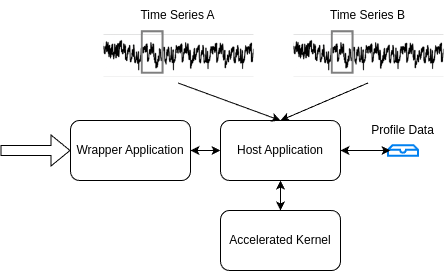
\includegraphics[scale=0.5]{architecture}
    \centering
    \caption{Architecture}
\end{figure}

The number of iterations of \texttt{Host Application} is dependant on the number of \texttt{Tiles} required to be processed and the size of the timeseries.

As outlined in Figure 3.1, the computation can be divided into four distinct phases:
\begin{enumerate}
    \item \textbf{Configure Run} \texttt{Wrapper Application}: Configures the parameters for the run. Decides the \texttt{Tile Size} and \texttt{Window} and the dimensions of the \texttt{Resource Rectangle} to be allocated for the run and splits the problem space into smaller chuncks which can be executed by the \texttt{Resource Rectangle}.
    \item \textbf{Pre-Computation} \texttt{Host Application}: The Host Application picks up the configuration from the Wrapper After the input time series is read, the statistics, i.e., $df, dg, $ and the L2-norms inverses are computed. The Host Application also computes the kernel arguments for each \texttt{Tile}. The host application also initializes the Simulator/Hardware and specifies the code to be pushed to the PEs that are part of the \texttt{Resource Rectangle}
    \item \textbf{Computation} \texttt{CSL Kernel}: Once the data is transfered, The Host Application calls the \textit{compute} function which triggers the computation on all PEs allocated in the \texttt{Resource rectangle}. After all tiles have successfully been
    computed by the kernel, the data is returned to the Host Application.
    \item \textbf{Post Computation} \texttt{Host Application} The next step in the computation is to merge the MP and MPI results from the tiles into a single Matrix Profile.
\end{enumerate}


\subsection{CSL Kernel}

Cerebras Software Language, or CSL is similar to syntax of Go, Swift and Scala.
It is designed for writing high-performance programs for PEs on the WSE. CSL is a medium-level language, in that it exposes both low and high-level programming features. CSL is low-level in
that it exposes the capabilities of the instruction set and some of the hardware structures that the
ISA controls. On the other hand, CSL is a high-level language in that it supports structured control
flow, loops, if-then-else constructs, and hides processor registers, performing automatic register
allocation. CSL allows for compile time execution of code blocks that take compile-time constant
objects as input, a powerful feature it inherits from Zig, on which CSL is based. CSL will be largely
familiar to anyone who is comfortable with C/C++, but there are some new capabilities on top of
the C-derived basics.\\

The main entry point to a CSL program is through defining the \texttt{Resource Rectangle} for the given program as depicted in Figure 3.2.
This specifies the number of PEs that needs to allocated for computation as detailed in Figure.
The language also allows us to flexibily specify the code to be pushed into a specific PE that can be executed during runtime of the program.
For our usecase, we have a single kernel implementation that is being pushed into every single PE that is allocated for the given computation.
Below is a piece of code that allocates a \texttt{Resource Rectangle} of size \texttt{WIDTH}, \texttt{HEIGHT} and pushes the code \texttt{tile\_kernel.csl} to each of the PE.
There is also the provision to pass params to each PE and the ability to modify them based on the requirements.\\

\clearpage
\begin{lstlisting}
    @set_rectangle(WIDTH, HEIGHT);
    for (@range(i16, WIDTH)) | x | {
      for (@range(i16, HEIGHT)) | y | {
          @set_tile_code(x, y, "tile_kernel.csl", .{ 
              .memcpy_params = memcpy.get_params(x),
              .LEN = LEN,
              .WINDOW = WINDOW,
              .N = LEN - WINDOW + 1,
          });
      }
  }
\end{lstlisting}

We will go over the main kernel algorithm in the upcoming Subsection 3.3 that is implemented on the device.

\subsection{Host Application}

The \texttt{Host Application} provides a path to the binaries created by the CSL compiler and specifies the name of the (simulated/real hardware)
core that should be written to post simulation. Once the application has finished running
on the simulator, the host reads the result from the core. The result is then stored onto a file for later comparing it's accuracy.\\

The Host Application also prepares the variables \(inv, df, dg\) for computation and concatenates the required data into a single array that is then pushed onto the device and spread across the allocated PEs.

\subsection{Wrapper Application}

The Wrapper Application is a wrapper of the \texttt{Host Application} and allows flexible execution of different tile sizes, partial matrix profiles and different \textit{CSL Fabric} configurations

\section{Kernel Design}

\subsection{Vanilla Kernel}

The \texttt{Vanilla Kernel} employs the update formulation described in Equation 2.6 by iteratively computing parts of the distance matrix contained within the current diagonal chunk. The entire entire execution of the Vanilla Kernel is contained within a single unit of execution. Its concept is rather simple, and it provides a good foundation to explain the \texttt{Tiled Kernel} in the following subsection. Subsequently, we describe the computation performed by the Vanilla Kernel:

\begin{enumerate}
    \item First, the initial set of QT values is used to initialize the internal variables (line 1). Additionally, the local aggregate representations are initialized (lines 2 - 3). As we calculate Pearson correlations instead of the Euclidean distances, as described in the previous section, aggregates are initialized with $-\infty$ instead of $\infty$.
    \item Next, the incremental update formulation, as described in Equation 2.6, is utilized to compute successive QT rows (line 7), and Equation 2.3 is employed to determine the Pearson correlation (line 8). Subsequently, the aggregates are updated accordingly (line 9 - 12).
    \item Once all diagonals within the current chunk have been computed, the aggregates are returned (line 15).
\end{enumerate}

Pseudocode for the Vanilla Kernel can be found in Algorithm 2.

\begin{algorithm}
\caption{Vanilla Kernel}\label{alg:Vanilla Kernel}
    \hspace*{\algorithmicindent} \textbf{Input} : Time Series $T$ of length \( n \in \mathbb{N} \) and subsequence length  \( m \in \mathbb{N} \) \\
    \hspace*{\algorithmicindent} \textbf{Output} : Matrix Profile $MP$ and Matrix Profile Index $MPI$
    \begin{algorithmic}[1]
        \State $df,dg,inv \gets PreComputeStatistics(T, m);$
        \State $QT_{init} \gets PreComputeInitialQTRow(T, m);$
        \State $rowAggregates, columnAggregates \gets (-\inf, -1);$
        \For{$iteration \gets 0$ \textbf{to} $\lceil \frac{n - m + 1}{1} - 1 \rceil$}
            \State $iteration_i \gets MatrixProfileKernel(QT_{init}, $df$, $dg$, $inv$);$
            \State $UpdateAggregates(rowAggregates, columnAggregates, iteration_i);$
        \EndFor
        \State $PostCompute(rowAggregates, columnAggregates);$\\
        \Return $MP, MPI;$
    \end{algorithmic}
\end{algorithm}
    
\subsection{Tiled Kernel}

SCAMP improves on the vanilla kernel for exploiting the parallelizable nature of the problem by implementing a systolic array architecture as described in Subsection 2.2.2.
As explained in Equation 2.6, the computation of $QT_{i,j}$ solely requires the QT value diagonally above ($QT_{i-1, j-1}$) and precomputed statistics, enabling every diagonal to be computed independently.
This can be exploited by instantiation multiple processing elements, of which each computes a set of $t$ (tile size) diagonals independently.
Therefore, the \texttt{Tiled Kernel} subdivides the diagonal chunk once again.
In constrast to the initial division, which aimed to decouple the problem size from the concrete kernel implementation, this subdivision exploits inherent parallelism. This division is visualized in Figure 3.3.\\

Every processing elements keeps track of it's row- and column-wise aggregates (lines 17 - 4) and update them accordingly,
similar to the Vanilla Kernel (lines 10 - 13). After all processing elements have completed their computation,
the individual aggregates can be reduced into a single set of aggregates (lines 16 - 22) which are subsequently returned.\\

\clearpage

\begin{algorithm}
    \caption{SCAMP Tiled Algorithm}
    \label{scamp_tiled_algorithm}
    \hspace*{\algorithmicindent} \textbf{Input} : The current Iteration $i$, $\overline{QT}_{init}$, as well as $df$, $dg$ and $inv$.\\
    \hspace*{\algorithmicindent} \textbf{Output} : Row- and Column-Wise Aggregates for the current \textbf{Diagonal Chunk}
    \begin{algorithmic}[1]
        \For{$ProcessingElement \gets 0$ \textbf{to} $\lceil \frac{w}{t}\rceil - 1$}
            \State $rowAggregates_{ProcessingElement} \gets (-\infty, -1);$
            \State $columnAggregates_{ProcessingElement} \gets (-\infty, -1);$
            \For{$row \gets 1$ \textbf{to} $h_i$}
                \For{$k \gets 1$ \textbf{to} $t$}
                    \State $column \gets i \cdot w + ProcessingElement \cdot t + row + k - 1;$
                    \State $QT_k \gets QT_k + df_{row} \cdot dg_{column} + df_{column} \cdot dg_{row};$
                    \State $P \gets QT_k \cdot inv_{row} \cdot inv_{column};$
                    \If{$P$ > is $rowAggregate_{ProcessingElement, row}.value$}
                        \State $rowAggregate_{ProcessingElement, row} \gets (P, column);$
                    \EndIf
                    \If{$P$ > is $columnAggregate_{ProcessingElement, column}.value$}
                        \State $columnAggregate_{ProcessingElement, column} \gets (P, row);$
                    \EndIf
                \EndFor
            \EndFor
        \EndFor
        \State $rowAggregates \gets (-\infty, -1);$
        \State $columnAggregates \gets (-\infty, -1);$
        \For{$ProcessingElement \gets 0$ \textbf{to} $w * h$}
            \State $Merge(rowAggregates, rowAggregates_{ProcessingElement});$
            \State $Merge(columnAggregates, columnAggregate_{ProcessingElement});$
        \EndFor\\
        \Return $rowAggregates, columnAggregates;$
    \end{algorithmic}
\end{algorithm}

Porting the SCAMP C++ Matrix Profiling Kernel to the Cerebras WSE engine presented several significant challenges, primarily stemming from the fundamental differences in architecture between conventional CPUs/GPUs and the specialized wafer-scale integration of the Cerebras device. The initial hurdle we encountered was defining the appropriate parameters and effectively distributing the workload onto the smaller processing elements (PEs) inherent to the Cerebras WSE architecture.

One of the foremost challenges lay in reconciling the intricacies of the SCAMP codebase, originally optimized for CPUs and GPUs, with the unique features and constraints of the Cerebras WSE. The SCAMP algorithm was intricately tailored to leverage specific compiler optimizations and architectural characteristics of conventional computing platforms, rendering direct translation to the Cerebras environment non-trivial. Thus, comprehensive modifications and optimizations were essential to ensure compatibility and performance efficiency on the novel hardware architecture.

In order to parallelize the Matrix Profile algorithm, the entire distance matrix calculated using Equation 2.9 is divided into square tiles of a maximum tile size. For a one-dimensional time series where the point of interest lies only in the tiles in the upper diagonal, the number of tiles \(T\) in SCAMP is calculated using the formula:


\begin{equation}
    T = \frac{N \cdot (N + 1)}{2}
\end{equation}

where:
\[
N = \frac{S}{T.S}
\]

where $S$ is the size of the time series and $T.S$ is the maximum size of the tile.


\begin{figure}[h!]
    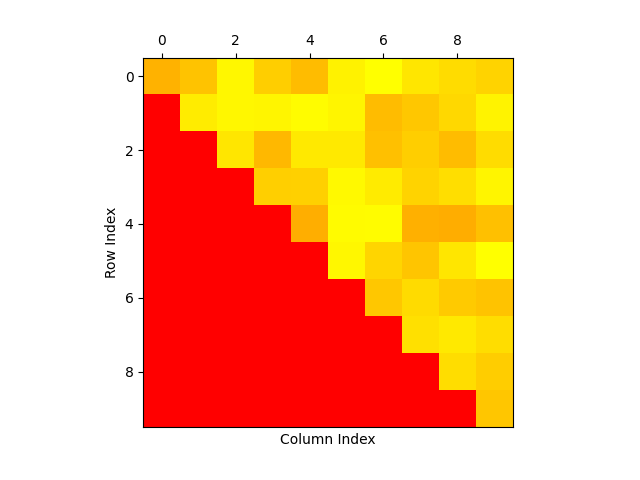
\includegraphics[scale=0.5]{tiling}
    \centering
    \caption{Tiling Representation}
\end{figure}

Rather than computing the entire distance matrix in one operation, we split it into tiles . Each tile independently computes
an AB-join between two segments of the input time series. This
allows the computation to scale to very large input sizes and
distribute the work to many independent machines
We finally settled on the following algorithm which is similar to the stripped down version of the SCAMP cpp implementation. Similar to the SCAMP version, The Statistics (\(df, dg, inv\)) are computed on the Host Device and then along with the Time series \(T_a, T_b\), passed on to the Device and distributed across the allocated \texttt{Resource Rectangle}. Once each device has recieved data, then the kernel computation is triggered from the host. Each PE is responsible to compute the aggregates for the particular tile since there are no data dependencies across tiles. The aggregates are then reduced on the host device. This was a design decision made given the constraint on the Cerebras system for communication across PEs.

\begin{algorithm}
    \caption{Cerebras Tiled Algorithm}
    \label{tiled_algorithm}
    \hspace*{\algorithmicindent} \textbf{Input} : Time series $T_a$, $T_b$, $df$, $dg$, $inv$ and $args$ for current \textbf{Tile}.\\
    \hspace*{\algorithmicindent} \textbf{Output} : Row- and Column-Wise Aggregates for the current \textbf{Tile}
    \begin{algorithmic}[1]
        \For{$ProcessingElement \gets 0$ \textbf{to} $w * h$}
            \State $rowAggregates_{ProcessingElement} \gets (-\inf, -1);$
            \State $columnAggregates_{ProcessingElement} \gets (-\inf, -1);$
            \Comment{Compute only top triangle}
            \State $QT \gets computeQT(T_a, T_b);$
            \For{$row \gets  0$ \textbf{to} $min(args.n_x - args.exclusion\_lower, args.n_y)$}
                \For{$diag \gets args.exclusion\_lower$ \textbf{to} $min(args.n_x - args.exclusion\_upper + 1, args.n_x - row)$};
                    \State $col \gets row + diag;$
                    \State $correlation \gets QT_{diag} \cdot inv_{row} \cdot inv_{col};$
                    \If{$correlation$ $>$ $rowAggregate_{ProcessingElement, row}.value$}
                        \State $rowAggregate_{ProcessingElement, row}.value \gets (correlation, column);$
                    \EndIf
                    \If{$correlation$ $>$ $rowAggregate_{ProcessingElement, column}.value$}
                        \State $rowAggregate_{ProcessingElement, column}.value \gets (correlation, row);$
                    \EndIf
                \EndFor
            \EndFor
        \EndFor
        \State $rowAggregates \gets (-\inf, -1);$
        \State $columnAggregates \gets (-\inf, -1);$
        \For{$ProcessingElement \gets 0$ \textbf{to} $w * h$}
            \State $Merge(rowAggregates, rowAggregates_{ProcessingElement});$
            \State $Merge(columnAggregates, columnAggregate_{ProcessingElement});$
        \EndFor\\
        \Return $rowAggregates, columnAggregates;$
    \end{algorithmic}
\end{algorithm}

Above is the final version of the Cerebras Tiled Kernel. It only implements computing the aggregates for one half of the triangle but the other half is computed by flipping the parameters hence computing the whole tile.
We also explored other version of tiling on the Cerebras to see if they offer any benefit 
\clearpage
% TODO: Images.
\section{Tiling Approaches}
\subsection{Trapezoidal}

While we were looking at different tiling approaches to experiment on its impact on the performance and efficiency, we looked at Trapezoidal tiles which in theory has the same area as a square but does not allow us to elegantly handle border conditions where there are a small section or the tiles on the diagonal which contain only a upper triangle.  

\subsection{Triangles}

Since we already have squares, the natural next step was to explore the implication of Triangle tiles. Although the kernel already supports triangles, The deconstruction of squares into rectangles leads to more jobs to be distributed across the Cerebras WSE. This also has an implication on the size of the \texttt{Resource Rectangle} since the number of triangles in the upper diagonal of the \textit{Distance Matrix} is more than the number of squares when deconstructed, this leads to more resource consumption but lesser execution time. This also has an impact on the memory transfer time to and from the device since a square tile and 2 triangles require the same amount of data and require reduction across two different PEs.

\section{Resource Allocation}

\subsection{Rectangle}

\begin{itemize}
    \item Memory Bus on the right side of the wafer of size 16. spread across the height. We noticed a improvement in memory transfer speeds when the PEs were spread across the height.
\end{itemize}

\subsection{Square}

\begin{itemize}
    \item Need to do more experiments to get values
\end{itemize}


\section{Scheduling}

Given the 745,500 available PEs on the Wafer, we are limited to the size of time series we can compute in a single run. This is also aggregevated by the fact that we have a soft limit on the maximum \texttt{Tile Size} that can be allocated on a single PE of 100.
Given that real world time series data sets can go in order of Billion entries \cite{8}, We explore here the different scheduling approaches to compute large scale time series data efficiently. 

\subsection{One Shot}

From Equation 3.1, We arrive at the total number of tiles that need to be computed for a given matrix of size $S$, When it is lesser than the allocatable number of PEs on the wafer/simulator, we can execute the entire Matrix Profile in a single iteration or \textit{One Shot}

\begin{figure}[h!]
    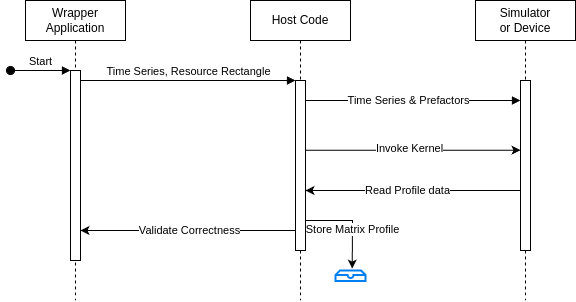
\includegraphics[scale=0.5]{job}
    \centering
    \caption{One Shot Execution of a small Time Series}
\end{figure}

The advantage of \textit{One Shot} scheduling is the reduced overhead of PE allocation and fewer memory transfer. In Practice, we found 
\subsection{Iterative}

\begin{figure}[h!]
    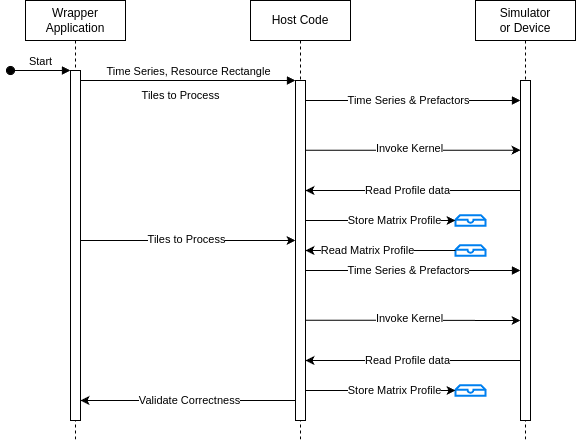
\includegraphics[scale=0.5]{iterative_job}
    \centering
    \caption{Iterative Execution of a large Time Series}
\end{figure}


\begin{itemize}
    \item Time Series of lower sizes have a smaller matrix profile.
    \item Generates tiles of maximum size 100 which can fit in the available fabric.
\end{itemize}
